\documentclass[12pt]{article}
\usepackage[utf8]{inputenc}
\usepackage{array}
\newcolumntype{C}[1]{>{\centering\let\newline\\\arraybackslash\hspace{0pt}}m{#1}}
\usepackage[spanish]{babel}
 \usepackage{url}
\usepackage[spanish, fixlanguage]{babelbib}
\bibliographystyle{IEEEtran}
\usepackage{graphicx}
\graphicspath{ {./images/} }

\title{Reporte del desarrollo de una Ontología}

\author{
	Saul Ivan Rivas Vega \\
	Inteligencia Artificial\\ 
}

\date{\today}

\begin{document}
	\maketitle
	
	\section{Introducción}
	Una definición para ontología es una descripción formal y explícita de conceptos, sus propiedades y las relaciones entre ellos. ~\cite{ontology_101}. En este trabajo se presenta 'Audio Subset'. Una ontología para la clasificación de eventos acústicos.\\
	Actualmente ha proliferado el interés de realizar un análisis en los distintos eventos sonoros en el ambiente con varios propósitos tales como el determinar el contexto para sistemas de agentes o una simple identificación de eventos en un extracto de sonido ~\cite{noauthor_computational_2017}. Así mismo existen una serie de tareas en las que se utilizan métodos de clasificación con uso de deep learning ~\cite{purwins_deep_2019}. Sin embargo es frecuente encontrarse con distintas categorizaciones para dichos eventos, casi una distinta con cada nuevo trabajo dependiendo el dominio ~\cite{eck_finding_2002, turpault_semi-supervised_2019, benetos_detection_2016}.\\
	Esto llevo a proponer una ontología al no existir una estándar. El trabajo resultante fue 'Audio Set' ~\cite{gemmeke_audio_2017}.
	De la cuál se obtuvo un subconjunto de las categorías para desarrollar 'Audio Subset', se describirá las diferencias con respecto a 'Audio Set' y algunos conceptos adicionales.
	\pagebreak
	\section{Desarrollo}
	\paragraph{}
	Buscaremos definir los siguientes conceptos
	~\cite{rae_2014}:
	\paragraph{Clase} Conjunto de elementos con caracteres comunes. 
	\paragraph{Propiedad} Atributo o cualidad esencial de alguien o algo.
	\paragraph{Característica} Que da carácter o que sirve para distinguir a alguien o algo de sus semejantes.
	\paragraph{}
	Ahora revisemos el subconjunto de 2 niveles de 'Audio Set':
	\\
	\begin{figure}[h]
		\centering
		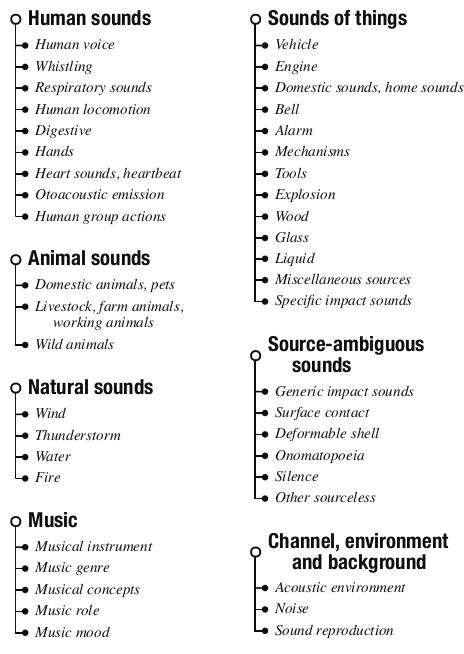
\includegraphics[width=0.55\textwidth]{audioSetOntology}
		\caption{Subconjunto como se muestra en ~\cite{gemmeke_audio_2017}.}
		\label{fig:audioOriginal Subset} 
	\end{figure}
	\paragraph{}
	Ademas de definir el 3er nivel y posteriores, se realizaron las siguientes modificaciones a los 2 primeros niveles:
	\begin{itemize}
		\item Cambiar el nombre de 'Hands' por 'Limbs', para generalizar el hecho de que el sonido puede provenir de la interacción de las extremidades y no solo de las manos.
		\item Dejar fuera 'Whistling' pues este puede entrar como instancia en alguna de las otras clases.
		\item Dejar fuera 'Octoacoustic emissions' pues realmente no es sonido detectable de manera externa (solo de manera interna en el oído).
		\item Dejar fuera 'Music Concepts' pues su definición es mas subjetiva ya que en la mayoría de la literatura se trabajan como características del sonido.
		\item Dejar fuera 'Music Mood' puesto que es determinado por una evaluación subjetivo de la emoción evocada por una pieza musical.
		\item Agregar 'Steel' a 'Sound of things' debido a que puede ser categorizado de igual forma que los demás materiales en la clase.
		\item Dejar fuera 'Miscellaneous sources' pues las entidades categorizadas carecían de similitudes significantes para ser agrupadas.
		\item Dejar fuera 'Specific Impact' pues las subclases no se diferenciaban mucho de 'Generic impact sounds' de la clase 'Source-ambiguous sounds'.
		\item Dejar fuera 'Onomatopoeia' pues son sonidos que hacen referencia a otros.
		\item Dejar fuera 'Silence' y 'Other sourceless' puesto que no se refieren a un sonido detectable.
	\end{itemize}
\pagebreak
\paragraph{}
\begin{figure}[h]
	\centering
	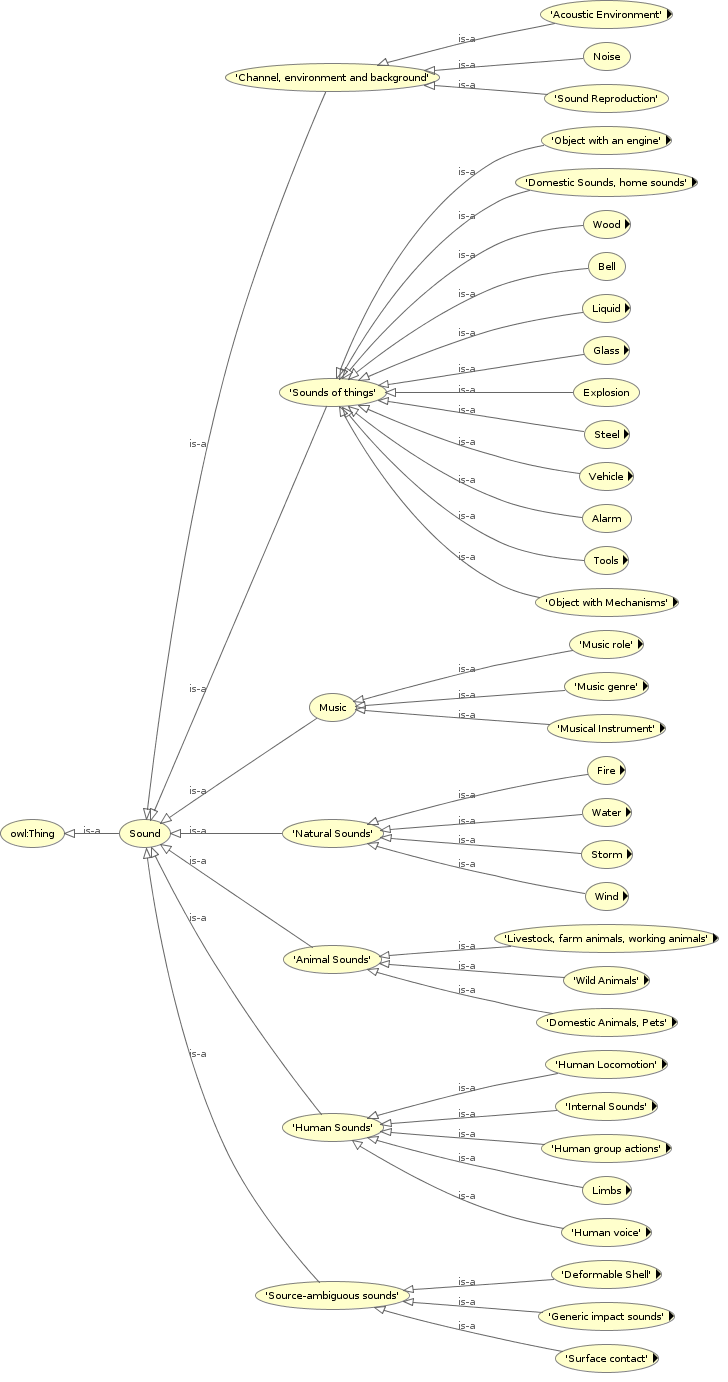
\includegraphics[width=0.535\textwidth]{visualization}
	\caption{Subconjunto de 2 niveles de Audio Subset.}
	\label{fig:audioSubset2} 
\end{figure}
\pagebreak
\section{Conclusiones}
\paragraph{}
El objetivo en el desarrollo de 'Audio Subset' como una exploración de las distintas categorizaciones en eventos acústicos se cumplió además de detectar las distintas modificaciones con respecto a la tarea a realizar. Se dejaron fuera varios eventos acústicos que no necesariamente son detectables, se entiende que 'Audio Set' los incluye pues es de una categorización mas general, y 'Audio Subset' trata de especificar las clases que sirvan para una aplicación práctica.
Finalmente el desarrollo de una ontología tiene gran valor como ejercicio en el aprendizaje sobre la representación del conocimiento con la finalidad de llevar a cabo una investigación en el dominio representado.
	\selectbiblanguage{spanish}
	\bibliography{main}
\end{document}